\documentclass[12pt]{article}
\usepackage{natbib}
\usepackage{pgf}
  \bibliographystyle{plainnat}
  \setcitestyle{citesep={,},aysep={}}
\usepackage[colorlinks,citecolor=blue,linkcolor=black,bookmarks=false,hypertexnames=true]{hyperref} 
\usepackage{url}
\usepackage[inline]{enumitem}
\usepackage{float}
\usepackage[bottom,perpage,multiple]{footmisc}
\usepackage{booktabs}
\usepackage{graphicx}
\usepackage{xcolor}
\usepackage{setspace}

\usepackage{enumitem}
\setlist{nosep}

  \setstretch{1.1}
\setlength{\bibsep}{0.0pt}
\tolerance=800

\usepackage{pgfplots}
%\DeclareUnicodeCharacter{2212}{-}
%\usepgfplotslibrary{groupplots,dateplot}
%\usetikzlibrary{patterns,shapes.arrows}
\pgfplotsset{compat=newest}

\usepackage{url}
\renewcommand*{\bibfont}{\footnotesize}

\title{Experiment with removing frequent patterns}
\author{Aibolit team}
\begin{document}
\maketitle
\newpage
\section*{Experiment}
According to previous experiments
patterns 'Non final class', 
'Non final attribute', 
'Null check' and 
'Var in the middle' 
are most frequent and important. 

\begin{figure}[h!]\center
	\begin{tabular}{cc}
		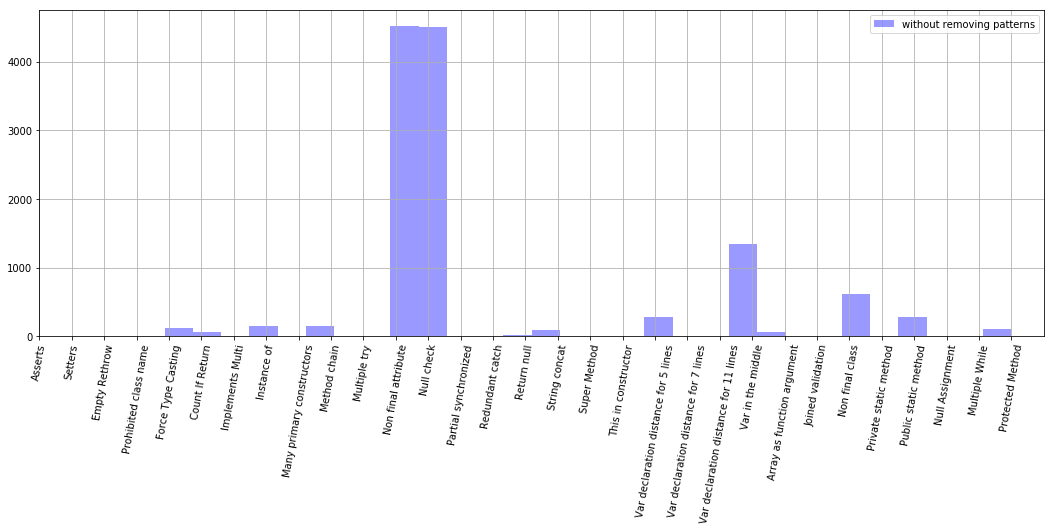
\includegraphics[scale=0.4]{3.png}
	\end{tabular}
	\caption{without removing patterns}
	\label{fig:ris3}
\end{figure}

In the experiment we trained
model without this patterns
and got best distribution of
patterns' importances. 
Our model predict pattern which
has the greatest impact on the
complexity. On the graphics
there is a distribution of 
most important
patterns. 

\newpage
Results of the experiment
are on the table.
\newline
p1 - remove pattern 'Non final class'
\newline
p2 - remove pattern 'Non final attribute'
\newline
p3 - remove pattern 'Null check'
\newline
p4 - remove pattern 'Var in the middle'
\newline

\begin{table}[h] \centering
\begin{tabular}{ | l | l | l | l |} 
	\hline
	Patterns & mse & mae & r2  \\ \hline
	no removing & 0.0182 & 0.0922 &  0.4792 \\ \hline
	p1 & 0.0181 & 0.0922 & 0.4811  \\ \hline
	p2 & 0.0195 & 0.0993 & 0.4395 \\ \hline
	p3 & 0.0209 & 0.1 & 0.4017 \\ \hline
	p4 & 0.0183 & 0.0932 & 0.4763 \\ \hline
	p1, p2 & 0.0196 & 0.0993 & 0.4366 \\ \hline
	p1, p3 & 0.0207 & 0.1 & 0.4052 \\ \hline
	p1, p4 & 0.0185 & 0.0935 & 0.4698 \\ \hline
	p2, p3 & 0.0228 & 0.1085 & 0.3453 \\ \hline
	p2, p4 & 0.02 & 0.1009 &  0.4259 \\ \hline
	p3, p4 & 0.0213 & 0.1016 & 0.3892 \\ \hline
	p1, p2, p3 & 0.0228 & 0.1087 & 0.3467 \\ \hline
	p1, p2, p4 & 0.02 & 0.1013 & 0.4264 \\ \hline
	p1, p3, p4 & 0.0214 & 0.1018 & 0.3874 \\ \hline
	p2, p3, p4 & 0.0235 & 0.1114 & 0.327 \\ \hline
	p1, p2, p3, p4 & 0.0237 & 0.1125 & 0.32 \\ \hline
\end{tabular}
\label{results}
\caption{Results of the experiment}
\end{table}
\newpage
\section*{Conclusion}
According to the results only removing one pattern 'Non final class' could improve quality of prediction complexity. 
\newline
More balanced distribution of patterns' importances is got in two cases:
\begin{itemize}
	\item removing all 4 patterns (\ref{fig:ris2})
	\item removing patterns 'Non final attribute', 'Null check' and 'Var in the middle' (\ref{fig:ris1})
\end{itemize}
But in this 2 cases quality of prediction reduced.
\newline
In sum, better to remove all 4 patterns because 
balanced distribution is more important than quality 
of prediction complexity.
\begin{figure}[h!]\center
	\begin{tabular}{cc}
		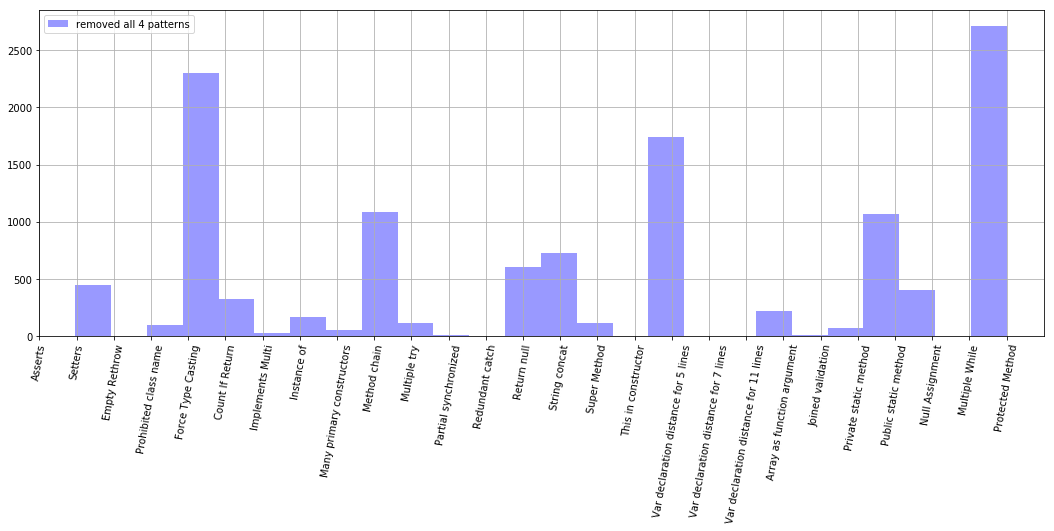
\includegraphics[scale=0.25]{2.png}
	\end{tabular}
	\caption{Removing all 4 patterns}
	\label{fig:ris2}
\end{figure}
\begin{figure}[h!]\center
	\begin{tabular}{cc}
		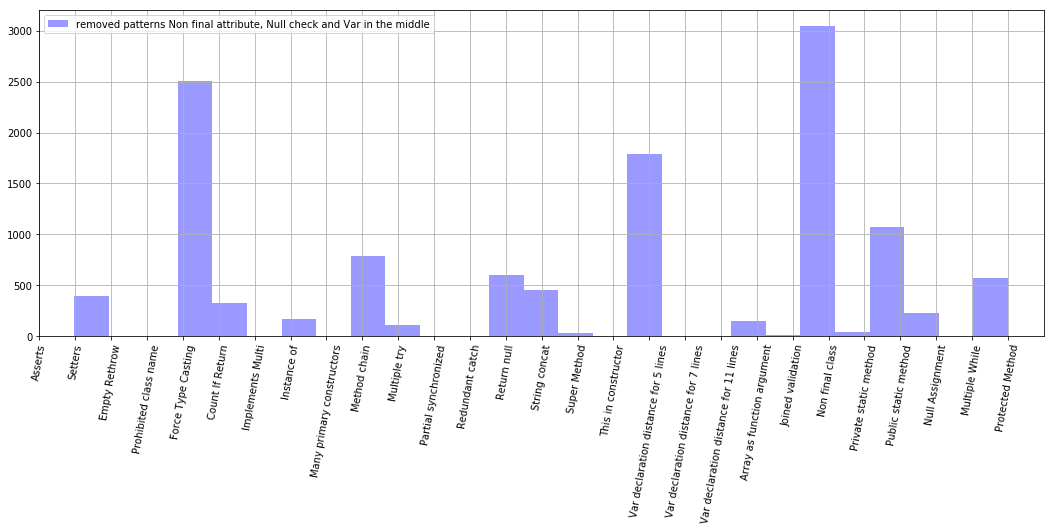
\includegraphics[scale=0.25]{1.png}
	\end{tabular}
	\caption{removing 'Non final attribute', 'Null check' and 'Var in the middle'}
	\label{fig:ris1}
\end{figure}
\end{document}